\chapter{Aprendizado de Máquina}
Como \citet{bishop2006pattern} descreve, aprendizado de máquina é uma maneira de abordar um problema de computação. Nessa abordagem, a partir de um grande conjunto de dados, chamados como conjunto de treinamento, são inferidos um conjunto de parâmetros a serem utilizados em um modelo parametrizado.

\section{Definições}

Algumas breves definições serão apresentadas para fim de ambientar o leitor nos temas discutidos neste capítulo.

\begin{description}
\item \textbf{Conjunto de exemplos}: Seja o conjunto de exemplos os dados conhecidos do problema.

\item \textbf{Características}: Sejam características um conjunto ordenado de valores que descrevem um exemplo, a ser modelada pelo algoritmo de Aprendizado.

\item \textbf{Etiquetas}: Seja etiqueta de exemplo, ou simplesmente etiqueta, a saída esperada do modelo para aquela instância.

\item \textbf{Acurária}: A proporção de acertos pelo tamanho do conjunto de exemplos.

\item \textbf{Precisão}: A proporção de exemplos inferidos corretamente como verdadeiros pela quantidade de inferidos como verdadeiro.

\item \textbf{Abrangência}: A proporção de exemplos inferidos corretamente como verdadeiros pela quantidade de acertos.

\item \textbf{\textit{F1 score}}: A média harmônica entre a precisão e a abrangência
\[\frac{2 * \mathrm{precisão} * \mathrm{abrangência}}{\mathrm{precisão} + \mathrm{abrangência}}\]

\item \textbf{Matriz \(\mathbf{X}\)}: Seja \(\mathbf{X}\), exemplos de treinamento, uma matriz \(m \times n\), o qual \(m\) é quantidade de instâncias e \(n\) é a quantidade de características. \(\mathbf{X}\) é a representação matemática do Conjunto de exemplos.

\item \textbf{Vetor \(\mathbf{Y}\)}: Seja \(\mathbf{Y}\), conjunto de etiquetas, um vetor de tamanho \(m\), a quantidade de instâncias, \(\mathbf{Y}\) é o conjunto ordenado das respectivas saídas esperadas de cada linha da matriz \(\mathbf{X}\), ou seja as etiquetas.
\end{description}

É importante destacar a relevância dos conceitos de precisão, abrangência e \textit{F1 score} para problemas que possuem poucos exemplos positivos. Essas definições permitem avaliar esses tipo de dados, como discutiremos na sessão de Detecção de Anomalias.

\section{Categorias de Problemas}

Para ser mais específico, é possível classificar os problemas resolvidos pela aprendizado de máquina em cinco categorias \citep{mohri2012foundations}.

\begin{description}
\item \textbf{Classificação}: Decidir a classe de exemplo dadas às suas características, por exemplo decidir qual dígito foi escrito a apartir de uma imagem de dígito escrita a mão.
\item \textbf{Regressão}: Determinar um valor real para cada exemplo, por exemplo o risco de um paciente ter contraído câncer a partir de imagens e resultados de exames.
\item \textbf{Ordenação}: Ordenar os exemplos a partir de algum critério, por exemplo listar produtos por relevância a partir das palavras chaves da busca do usuário.
\item \textbf{Agrupamento}: Particionar os exemplos em regiões homogêneas, por exemplo identificar comunidades dentro de redes sociais massivas.
\item \textbf{Redução de Dimensionalidade}: Representar o conjunto de exemplos com um número reduzido de dimensões, por exemplo comprimindo imagens para processamento de imagens.
\end{description}

Neste projeto o objetivo é identificar grupos com padrão de comportamento semelhantes. A expectativa é que o comportamento dos bots formem grupos divergentes dos usuários legítimos. Todavia, nem toda máquina pertencente a esse grupo divergente está infectada, o que se quer garantir é um número de reduzido, não mais que 100, de máquinas suspeitas para serem analisadas.

\section{Cenários dos Dados}

Categoriza-se \citep{mohri2012foundations} sete cenários para os algoritmos de aprendizado, esse cenários são fortemente influenciados pelas condições dos dados de treinamento.

\begin{description}
\item \textbf{Aprendizado Supervisionado}: O modelo tem acesso a dados com os resultados de saída já esperados, ou etiquetados, como lê-se na literatura. Os problemas mais comuns desse tipo de cenário são classificação, regressão e ordenação.

\item \textbf{Aprendizado Não Supervisionado}: Só se dispõe da conjunto de exemplos para treinamento sem etiquetas. Geralmente é mais utilizado para classificação, agrupamento e redução de dimensionalidade

\item \textbf{Aprendizado Semi-Supervisionado}: Neste cenário, é possível acessar uma conjunto de exemplos sem etiquetas e uma com etiquetas. Esse é o caso de problemas em que dados sem etiquetas são fáceis de serem adiquiridos, ao contrário dos dados etiquetados, pela dificuldade de etiquetar.

\item \textbf{Inferência Transdutiva}: Semelhante ao Aprendizado Semi-Supervisionado, nem todos os exemplos são etiquetados, mas o modelo só deve ser generalizado apenas para os exemplos conhecidos.

\item \textbf{Aprendizado On-line}: Neste cenário, iterasse no modelo a cada exemplo recebido em rodadas. No início da rodada, o modelo recebe um exemplo, inicialmente sem etiqueta, realiza uma predição, recebe a etiqueta e atualiza os parâmetros do modelo.

\item \textbf{Aprendizado por Reforço}: Neste cenário, os modelos são criados baseado num sistema de recompensa. O modelo é recompensado a cada decisão bem-feita ao interagir com um ambiente.

\item \textbf{Aprendizado Ativo}: O algoritmo é quem realiza requisições a uma entidade capaz de etiquetar exemplos para melhorar os parâmetros do modelo. O objetivo é conseguir gerar um modelo tão bom quando o modelo supervisionado, porém com menos exemplos.

\end{description}

E ainda há outros possíveis cenários ainda mais complexos e específicos. Esses cenários não foram catalogados neste trabalho porque a campo de Aprendizado de Máquina está ainda em constante fase de crescimento.

No caso deste trabalho, algumas máquinas identificadas pelo IP foram confirmadas como bots, mas não há garantia de que sejam os únicos bots na rede. O algoritmo se vê num cenário não supervisionado, mas os desenvolvedores validam os resultados a partir dos bots já conhecidos.

Note que se as máquinas conhecidamente suspeitas não se encontrarem no grupo divergente, o sistema falhou.

\section{\textit{K-Means}}

Segundo \citet{witten2011data}, \textit{K-Means} é um algoritmo de aprendizado iterativo baseado na distância geométrica. Inicialmente o algoritmo inicializa \textit{K} centróides em posições distintas. Cada exemplo, então, é associado ao centróide mais próximo. Em seguida o centróide atualiza sua posição para a média das posições dos pontos associados a ele. A partir de então recomeça o ciclo, são reassociados os pontos que estão mais próximos do centroíde em sua nova posição.

\begin{figure}
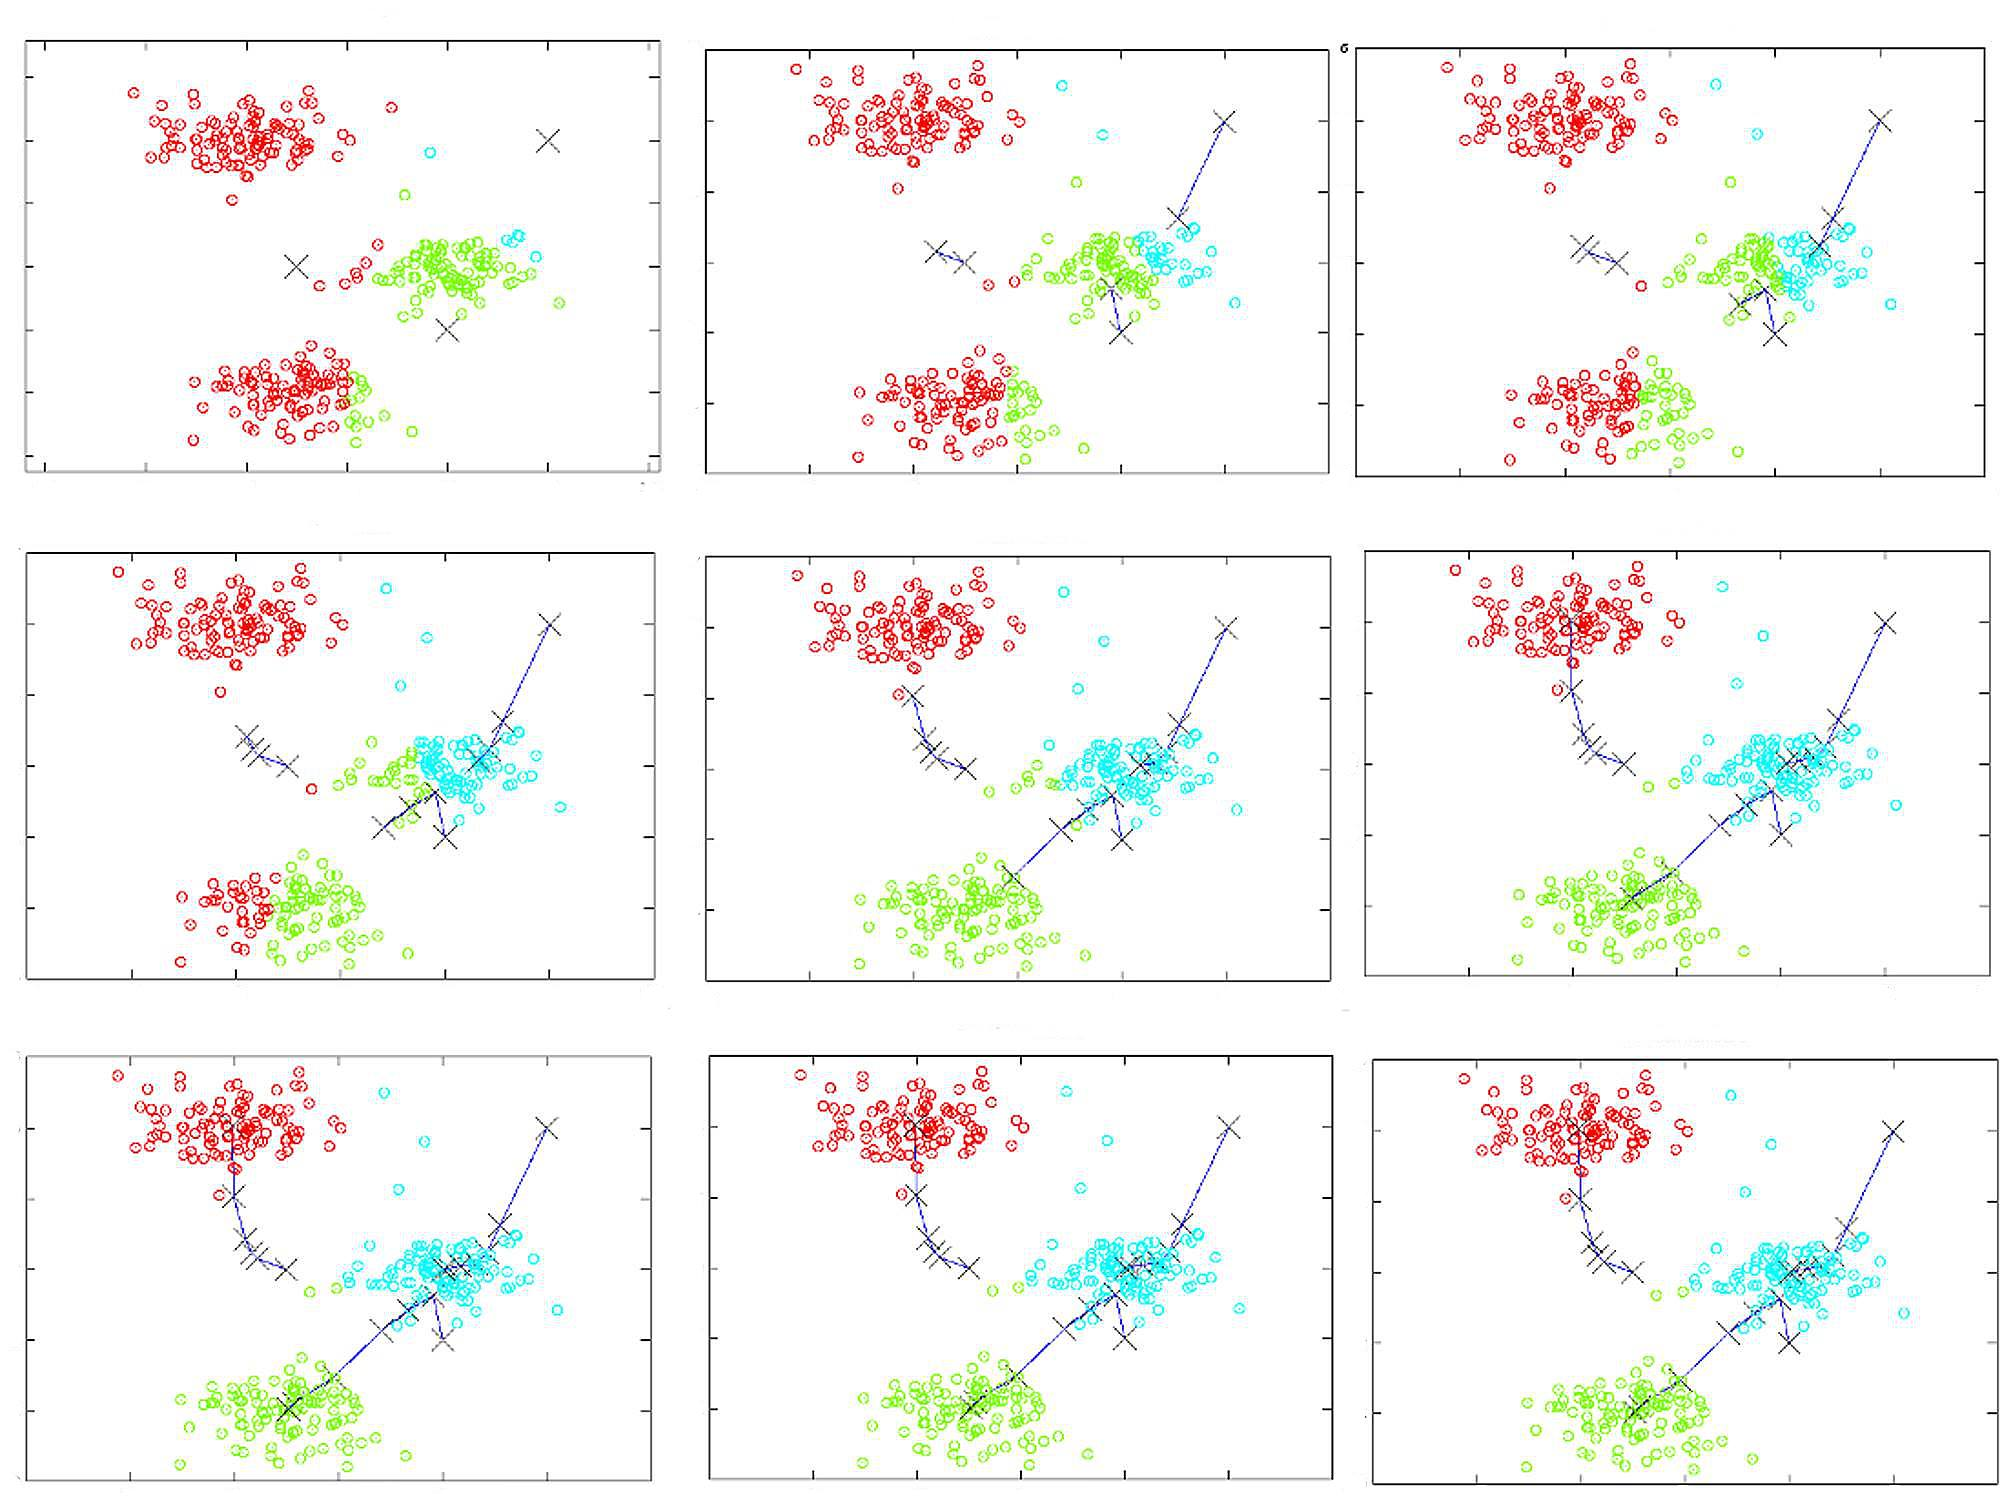
\includegraphics[width=\textwidth]{k_means_example}
\caption[Aplicação do K-Means]{Aplicação do K-Means} \label{fig:k_means_example}
\end{figure}

A \ref{fig:k_means_example} representa a aplicação da técnica em dados bidimensionais com três grupos. É possível notar que converge rapidamente, nesse caso em apenas 9 iterações chegou-se a um resultado satisfatório. Além disso, espera-se uma quantidade de máquinas da ordem de \(10^4\), como o algoritmo \textit{K-Means} é linear tanto na decisão do cluster para cada instância quanto no cálculo do novo centróide.

\subsection{Determinação do Número de Grupos}

Para a operação plena do algoritmo é necessário que seja informada a quantidade de grupos que são buscados. Isso pode ser um problema simples quandos é possível visualizar os dados, como na figura \ref{fig:k_means_example}, mas não é possível realizar o mesmo procedimento quando os exemplos têm mais que três dimensões, como no caso deste projeto.

\begin{figure}
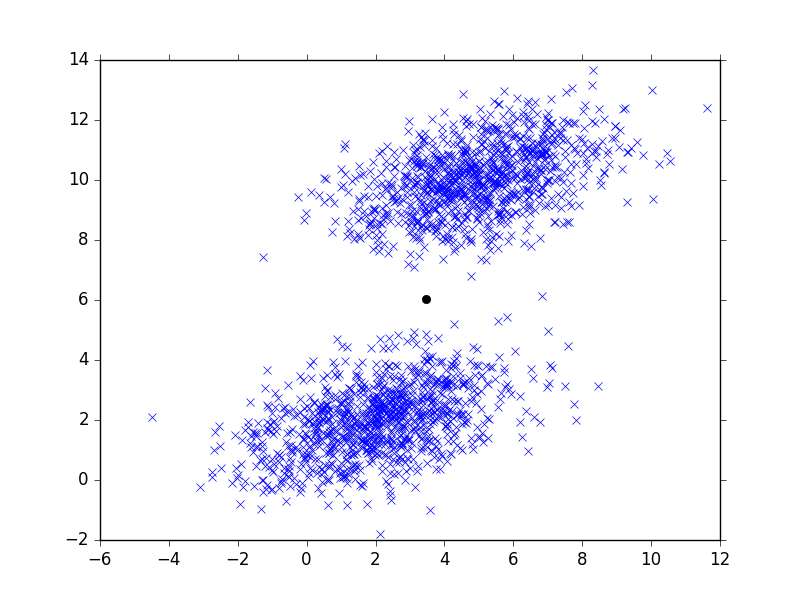
\includegraphics[width=\textwidth]{between_two_clusters}
\caption[Centróide Pouco Representativo]{Centróide Pouco Representativo} \label{fig:between_two_clusters}
\end{figure}

Além disso, se por um lado, pode-se carecer centróides levando a cenários como na figura \ref{fig:between_two_clusters}, no qual o centróide não generaliza os dados, por outro, como é possível visualizar na figura \ref{fig:cluster_overfitting}, um grupo pode acabar se separando centróides desnecessários.

\begin{figure}
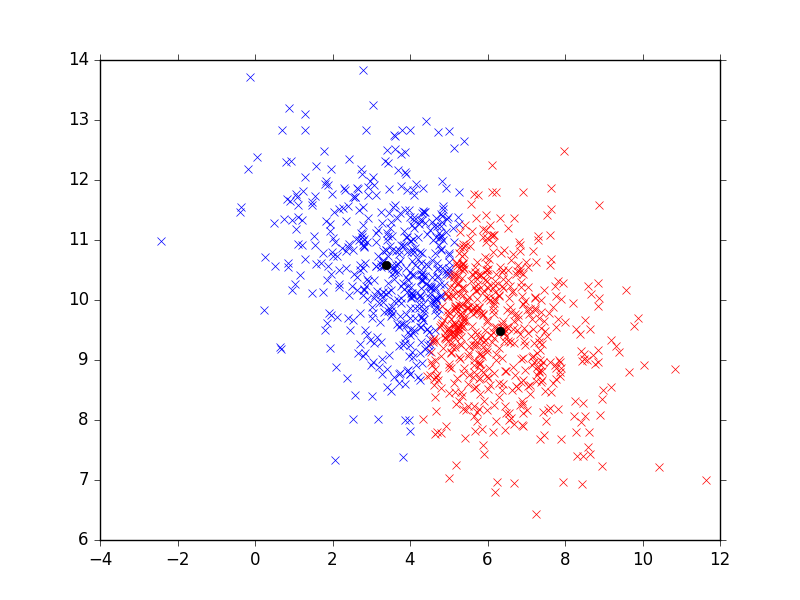
\includegraphics[width=\textwidth]{cluster_overfitting}
\caption[Grupo Dividido]{Grupo Dividido} \label{fig:cluster_overfitting}
\end{figure}

Para resolver esse problema utiliza-se o Método \textit{Elbow} \citep{kodinariya2013review}. Trata-se de um método visual no qual procura-se o ponto em que a adição de um novo centróide não implica mais na redução drática da soma das distâncias entre os exemplos e seus respectivos centróides. Esse efeito é observado na figura \ref{fig:elbow}

\begin{figure}
\centering
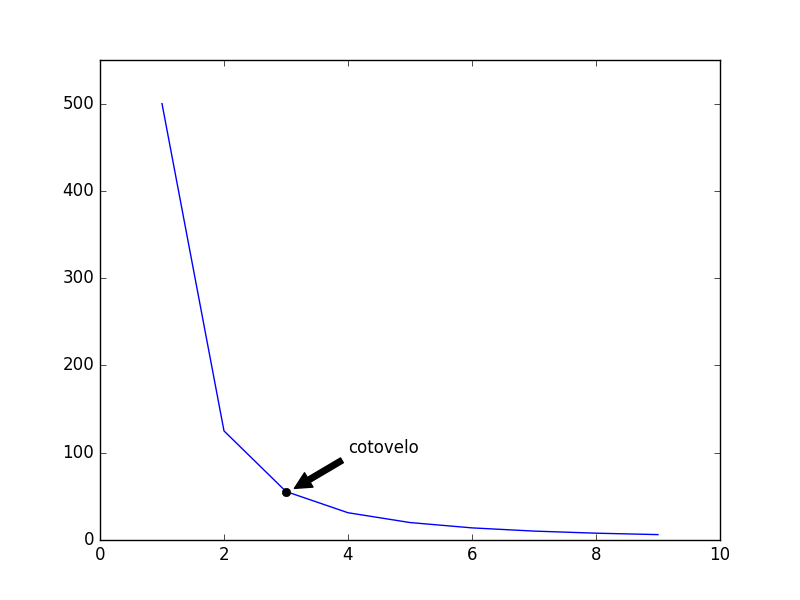
\includegraphics{elbow}
\caption[Ponto Crítico da Otimização]{Ponto Crítico da Otimização \citep{kodinariya2013review}} \label{fig:elbow}
\end{figure}

Dessa forma, evita-se os cenários das figuras \ref{fig:between_two_clusters} e \ref{fig:cluster_overfitting}.